\section{Технико-экономическое обоснование}
\subsection{Описание проекта}
\subsubsection{Резюме}

Бизнес план посвящен разработке и вывод на рынок сверхдешевого дельта-робота с оригинальным управлением. Стоимость самого робота в 50 тыс. руб., программное обесспечение к нему 300 тыс. руб.

Для фирмы требуется два специалиста с начальным уровнем зарплаты в 105 тыс. руб.

Начальное капиталовложение не менее 600 тыс. руб.

Себестоимость одного робота может варьироваться, но принята за 7137 рублей.
При продаже за год 36-и роботов и 8 комплектов ПО, чистая прибыль составит 1583 тыс. руб. 

\newpage


\subsubsection{Описание продукции}
Готовым продуктом выступает паралельный робот, а конкретно легкий дельта-робот с грузоподьемностью не более одного килограмма. Данная машина востребована в широком спектре производственных задач, связанных с манипулированием материалами, сортировкой продукции или отбраковки. В виду своей конструкции может быть монтирован непосредственно над линией конвеера, занимает мало пространства.

Пример названия продукта:\\
Дельта-робот модель подвесная\\
Характеристики:\\
Количество осей: 3\\
Грузоподъемность: 1 кг.\\
Радиус действия: 300 мм.\\
Повторяемость: 2 мм.\\
Потребляемая мощность 200 Вт.\\
Вес: 4 кг.\\

Целью моего проекта было создание параметрической модели робота, с помощью которой можно относительно просто подобрать необходимые размеры будующего робота под нужды заказчика. Так как расчет рабочей области данного типа роботов является не тривиальной задачей, наглядная 3д модель, интерактивно меняющие свои параметры, такие как: радиус базы, форм-фактор шаговых двигателей, длины рычагов и шарниры, размеры каретки - является большим подспорьем. В сцену можно легко добавить объекты имитирующие будующее рабочее место робота, а анимация покажет, какие траектории он сможет совершать. Габариты и параметра робота можно и нужно менять до оптимальных для конкретного заказчиска, после чего только подходить к процессу создания самого продукта. Так как рабочая зона ограничена в радиусе проделываемой операции, персонал производственной линии может безопасно работать в непосредственной близости от робота.

Дельта-робот спроектирован для печати большинства своих деталей на 3д принтере, что позволяет сильно удешивить себестоимость изделия буквально во всем. Пластик не обладает высокой жесткостью, поэтому робот не обладает большой точностью позиционирования, что не мешает использовать его в задачах, переноса небольших объектов. Зато робот чрезвычайно прост в изготовлении, все его детали легко заменяемы, масштабируемы в любых пропорциях, для создания замены требуется только время.

Потенциальными покупателями могут выступать производители пищевой продукции, в операциях дозирования теста на жаровой поверхности, выдавливании кремов определенным рисунком или фасовке готовой продукции. Так как робот состоит большей частью из нейтрального пластика, без смазочных материалов, он способен работать непосредственно с пищей. Максимальная дешевизна робота может помочь его массовому внедрению в центры переработки мусор, где скромные технические показатели будут невелированы массовостью. По той же причине, робот можно использовать в качестве учебного пособия, поставляя его в школьные классы, молодежные кружки. Робот может служить умным освещением, следя за работой человека и освещая рабочее место в условиях, когда человек не может отвлечься.
\subsubsection{Анализ рынка сбыта}



\subsubsection{Анализ конкурентов}
\subsection{План маркетинга}
Интересующиеся данными технологиями могут быть завлечены с помощью демонтрации 3д моделей или видеороликов работы готовых моделей. Для этого следует заводить тематические каналы на видеохостингах, с наглядным описанием того, как это работает и как это можно использовать. Обязательно продемонстрировать работу с заказчиком, так как необходимо доказать, что пластиковые роботы способны совершать полезную работу и окупаться.
Основным рекламным ходом планируется использовать открытость продукта, рекламой будет служить возможность заказчику самостоятельно производить новых роботов. И конечно большую степень гибкости и возможность самостоятельного апгрейда.

Рекламировать роботов необходимо с сильным упором на общую "экологичность" пластмассовых механизмов, состоящих из пластика PetG - основного пластика для производства бутылок. Учавствующие в сортировке мусора роботы, могут быть частично или полностью состоять из отсортированных бутылок или другого вторичного материала. Рекламные ролики лучше всего распространять в тематических группах в социальных сетях, где обитают люди заинтересованные в самоделках, экологии и технологиях 3д печати. Например, групп: "Ветряки своими руками", "Зеленая энергетика", "Все о 3д печати", "Собираю ЧПУ станок" и подобные.

Также в рекламных чрезвычайно важно попасть на тематическую выставку:

- VendExpo и WRS5-2021 (15-я международная выставка вендинговых технологий и систем самообслуживания).

- RosBuild 2021 (Международная специализированная выставка строительных,отделочных материалов и технологий в рамках «Российской строительной недели-2021»).

- ЭЛЕКТРО-2021 (30-я международная выставка. Электрооборудование. Светотехника. Автоматизация зданий и сооружений).

В качестве сервисного ремонта следует предлагать бесплатную замену любых напечатанных частей, если поломка произошла в процессе эксплуатации, так как себестоимость таких частей примерно равняется стоимости пластика.

\subsubsection{Анализ рынка}

Прямые конкуренты на рынке не представлены, так как идея создания роботов из пластика витает в воздухе, но не доведена до ума. Конкурироавть необходимо со стандартными роботами, которые представляют собой устройства другого класса, с точностью позиционирования в 0.02 мм., огромным запасом по надежности и прочности. Но такие роботы стоят хороших денег.

\begin{figure}[h]
\centering
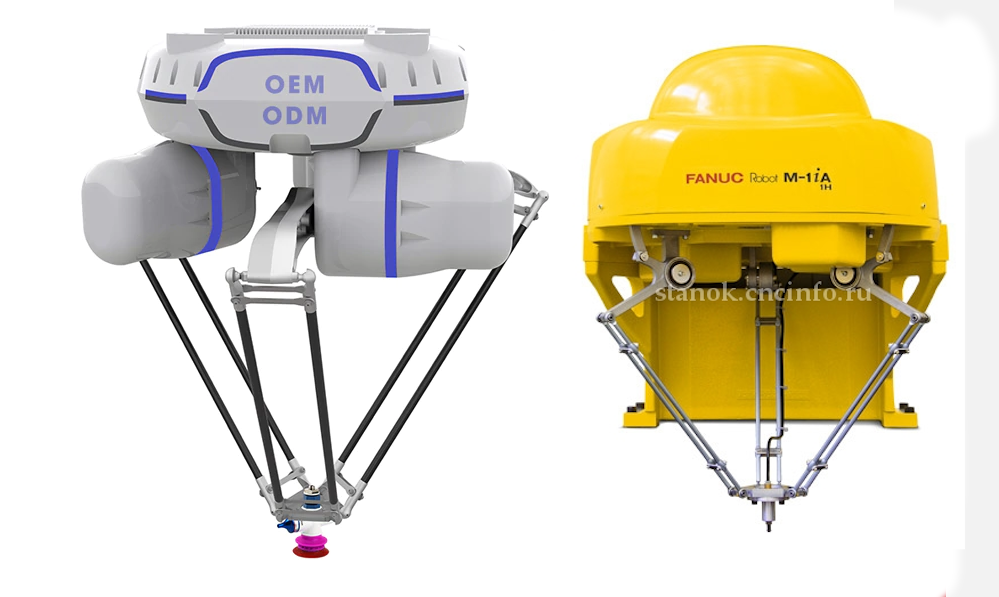
\includegraphics[width=0.8\linewidth]{./image/odm}
\caption{Примеры конкурентов на рынке}
\end{figure} 

Робот <<OEM ODM>> китайского происхождения, стоит 744 тыс. рублей, но без представительства в России. Робот <<Fanuc>> японского происхождения, но собирается в России. Стоимость зависит от заказчика, мне удалось выяснить, что начинается она от 600 тыс. руб. Оба робота имеют грузоподьемность в килограмм, высокую точность позиционирования, и массивную базу. У <<Fanuc>> база весит 17 кг., позволяя ему избегать вибраций, возникающих при работе. Данные роботы предназначены для чистых производств, маловероятно увидеть их на сортировке мусора. Ниша сверхдешёвых дельта-роботов на данный момент свободна, что связано со сложностью написания программного обепечения для управления паралельной машиной.

\subsubsection{Ценовая политика}

Основной статьей заработка следует считать разработку программного продукта для решения конкретной задачи, поставленной заказчиком. Так как свободное ПО для управления данным типом робота отсутсвует в принципе, программы придется писать в любом случае. Особенно в начале, когда не будет еще большого опыта и наработанной базы проектов. Поэтому за программый продукт логично брать больше, чем стоимость самого робота, более того, возможно, передать электроннные модели закачику.

\subsubsection{Сбытовая политика и мероприятия}
\begin{table}[h!]
    \centering
\begin{tabular}{|l|c|c|c|c|c|}
\hline
Показатели &\multicolumn{4}{|c|}{Квартал}   & Всего\\
\hline
           & I & II & III & IV & \\ 
\hline
\textbf{Разработка ПО}  & &  &  &  &  \\
\hline
Ожидаемы объем продаж, ед.  & 1  & 2  & 2  & 3  & 8  \\
\hline
Цена с НДС, т.р.  & 300  & 300  & 300  & 300  &  \\
\hline
Выручка с НДС, т.р.   & 300  & 600  & 600  & 900  & 2400 \\
\hline
Нетто-выручка (без НДС), т.р.  & 250   & 500  & 500  & 750  & 2000 \\
\hline
Сумма НДС, т.р   & 50  & 100 & 100  & 150  & 400 \\
\hline
\textbf{Дельта-робот}  & &  &  &  &  \\
\hline
Ожидаемы объем продаж, ед.  & 3 & 6  & 9  & 18  & 36  \\
\hline
Цена с НДС, т.р.  & 50  & 50  & 50  & 50  &  \\
\hline
Выручка с НДС, т.р.   & 150  & 300 & 450  & 900  & 1800 \\
\hline
Нетто-выручка (без НДС), т.р.  & 125  & 250  & 375  & 750  & 1500 \\
\hline
Сумма НДС, т.р   & 25   & 50  & 75  & 150  & 300 \\
\hline
\end{tabular}
\caption{План продаж}
\end{table}



\subsection{План производства}
                            
Группы комплектующих, из которых будет состоять система:\\
1) Комплектующие которые печатаются на 3д принтере: основные конструкционные детали, редуктор, шарниры, крепление, каретка и части рабочего органа.\\
2) Электроника, включающая в себя arduino cnc shield, драйвера двигателей A4988, шаговые двигатели, orange Pi, orange Pi camera, импульсный адаптер питания, концевики.\\
3) Силовые элементы, в качестве которых выступает квадратная алюминеевая труба 15х15 мм. и круглая алюминиевая труба 8 мм. В зависимости от требований заказчика, диаметры труб можно варьировать.\\
4) Прочие расходные материалы: подшипники, винты, самоконтрящиеся гайки, провода, стяжки.

Основной процесс изготовления заключен в печати деталей базы, последующей механической обработке (снятие поддержек, ошкуривание и подобное) и самого процесса сборки. Для печати выбран пластик PetG, как самый распространенный пластик, имеющий неплохие прочностные характеристики, не разлагающийся под действием ультрафиолета и работающего при температурах до $80^{\circ} C$. Конечно, возможен переход на промышленные пластики, показатели которых на совершенно ином уровне. Но это приведет к необходимости изменить геометрию деталей, сделать их более грацильными, так как во многих местах прочность будет излишняя.

\begin{table}[h!]
    \centering
\begin{tabular}{|l|c|c|c|c|c|}
\hline
Модель stl &  Время печати & Штук  & Расход г. & Общее время & Общий расход\\
\hline
basa  &  12h 58m & 1 & 132.77 & 12h 58m & 132.77 \\
\hline
krepej  &  11h 10m & 3 & 96.68 & 1d 9h 30m & 290.04\\
\hline
worm  &  3h 35m & 3 & 31.74 & 10h 45m & 95.22 \\
\hline
ploshadka1  &  3h 1m & 1 & 24.47 & 3h 1m & 24.47\\
\hline
ploshadka2  &  2h 53m & 1 & 24.21 & 2h 53m & 24.21\\
\hline
krep\_konch\_niz  &  31m & 3 & 3.92 & 1h 33m & 11.76\\
\hline
krep\_konch  &  30m & 3 & 3.97 & 1h 30m & 11.91\\
\hline
lokot\_verh  &  2h 18m & 3 & 24.18 & 6h 54m  & 72.54\\
\hline
lokot\_niz  &  37m & 12 & 6.68 & 7h 24m & 80.16\\
\hline
plecho\_krep  & 1h 26m & 3 & 11.56 & 4h 18m & 34.68\\
\hline
Итого:  &  &  &  & 3d 12h 46m & 777.76\\
\hline
\end{tabular}
\caption{Расход времени и пластика на печать деталей}
\end{table}

Время, приведенное в таблице 1, отображает минимальное время требуемое для печати, без учета времени на разогрев, постановку на печать следующей детали и возможных прерываний печати, связанных с застреванием филамента, плохой адгезией или сдвигом по слоям. Для достижния приемлеммых временных рамок, требуется использовать параллельную печать, минимум на 2 принтерах. При получении крупного заказа, выполнить его в разумные сроки будет возможно только при создании фермы из принтеров. 

\begin{table}[h!]
    \centering
\begin{tabular}{|l|c|c|c| }
\hline
Наименование & Штук & Цена за шт. руб.  & Стоимость руб. \\
\hline
Arduino Uno & 1 & 300 & 300 \\
\hline
Arduino CNC Shield & 1  & 250 & 250 \\
\hline
driver A4988 & 3  & 100 & 300 \\
\hline
Адаптер питания 500 Вт. & 1 & 1250 & 1250 \\
\hline
Orange Pi  с камерой & 1 & 1400 & 1400\\
\hline
Двигатели Nema 17 & 3  & 475  & 1425  \\
\hline
Концевой переключатель & 6 & 10  & 60  \\
\hline
Подшипник 5х8х2.5 & 6  & 32  &  192 \\
\hline
Труба квадратная 15х15 мм. 2м. & 1  & 200  & 200  \\
\hline
Труба круглая 8 мм. 1м & 2 & 80 & 160 \\
\hline
Винты и прочий крепеж & 1 & 300 & 300 \\
\hline
Филамент PetG кг.  &  1  & 1300 & 1300 \\
\hline
Итого: &  &  & 7137 \\
\hline
\end{tabular}
\caption{Стоимость расходников}
\end{table}

Под производства необходимо два помещения: офисное для проектирования и мастерская для сборки и печати. В офисе необходимо два компьютера:

- для менеджера по продажам и закупкам продукции

- рабочее место проектировщика с CAD-приложением, слайсером для 3d печати.

В мастерской необходимы:

- место электрика, оборудованное паяльными принадлежностями, набором коробок и стеллажей для комплектующих.

- верстак с рабочими инструментами, где можно будет скручивать соединения, обрабатывать детали, проводить сборку.

- место для размещения 3д принтеров.

Минимальная цена аренды промышленного помещения в 50 м.$^{2}$ в Санкт-Петербурге стоит около 40 тыщ. рублей в месяц. 480 тыщ. рублей в год.
\begin{table}[h!]
\centering
\begin{tabular}{|l|c|c|c|}
    \hline
    Наименование & Штук & Цена тыщ. руб.  & Стоимость тыщ. руб. \\
    \hline
    Автоматизированное рабочее место & 2 & 80  & 160 \\
    \hline
    3д принтер & 2 & 50  & 100 \\
    \hline
    Рабочее место электрика & 1 & 100 & 100 \\
    \hline
    Верстак с инструментом & 1 & 100 & 100 \\
    \hline
    Итого: &&& 420 \\
    \hline
\end{tabular}
\caption{Стоимость оборудования}
\end{table}

Основным процессом производства будет проектирование деталей, для реализации пожеланий заказчика и печать деталей. С двумя принтерами изготовление комплекта для одного робота должно укладываться в рабочее время 5-6 календарных дней. Разброс неизбежен, так как время зависит от размеров итоговых деталей. Для реализации большого заказа необходимо докупать дополнительные принтеры, либо отдавать печать на оутсорс в ателье 3д печати, что может рассматриваться, как очень выгодный вариант.

По моему мнению, необходимый персонал может состоять из двух человек, каждый из которых берет на себя сразу по две роли. Конечно, роли поделены достаточно условно, каждый должен быть готов подменить другого и понимать работу товарища.  

\begin{table}[h!]
\centering
\begin{tabular}{|l|c|c|c|}
    \hline
    Наименование & Ставка & Зарплата тыщ. руб.& Всего тыщ. руб. \\
    \hline
    Инженер проектировщик & 0.5 & 80  & 40 \\
    \hline
    Оператор 3д принтера & 0.5 & 50  & 25 \\
    \hline
    Электрик-сборщик & 0.5 & 50 & 25 \\
    \hline
    Менеджер по продажам & 0.5 & 50 & 25 \\
    \hline
    Итого зарплата в месяц: &&& 105 \\
    \hline
\end{tabular}
\caption{Первоначальный уровень зарплат}
\end{table}


\subsection{Финансовый план}

\begin{longtable}[c]{|p{110pt}|p{110pt}|c|c|c|c|c|}
\hline
Показатели & Источник информации  &\multicolumn{4}{|c|}{Квартал}   & Всего\\
\hline
& & I & II & III & IV & \\ 
\hline
1. Вырочка-нетто (без учета НДС) от реализации & План продаж  & 450 & 900  & 1050  & 1800  & 4200  \\
\hline
2. Переменные производственные затраты &  &  &  &  &  &  \\
\hline
2.1 Переменные материальные затраты & План материально-производственных затрат  & 21.411 & 42.822  & 64.233  & 128.466  & 256.932  \\
\hline
2.2 Переменные затраты на оплату труда & План затрат на оплату труда производственного персонала   & 315 & 315 & 315 & 315 & 1260 \\
\hline
2.3 Переменные общепроизводственные затраты  & План общепроизводственных затрат  & 540 & 120  & 120  & 120  & 480 \\
\hline
3. Валовая прибыль &  & 428.589 & 857.178  & 985.767 & 1671.534 & 4943.068  \\
\hline
4. Переменные управленческие и коммерческие затраты & План управленческих и коммерческих затрат  & 0  & 0  & 0 & 0 & 0 \\
\hline
5. Маржинальная прибыль &  &  &  &  &  &  \\
\hline
5.1 Разработка ПО  &   & 250  & 500  & 500 & 750  & 2000 \\
\hline
5.2 Дельта-робот &  & 103.589  & 257.178 & 385.767 & 771.534 & 1543.063  \\
\hline
6.1 Постоянные общепроизводственные затраты  & План общепроизводственных затрат  & 75  & 150 & 175  & 300  & 700  \\
\hline
6.2 Постоянные управленческие и коммерческие затраты & План управленических и коммерческих затрат  & 0 & 0 & 0 & 0 & 0 \\
\hline
7. Прибыль от продаж &  & 375  & 750 & 875  & 1500 & 3500  \\
\hline
8. Прибыль до налогооблажения & & 450  & 900 & 1050  & 1800  & 4200  \\
\hline
9. Налог на прибыль &  & 75  &  150  &  175 & 300 & 700 \\
\hline
10. Чистая (нераспределенная) прибыль &  & -626.411  & 422.178 & 550.767 & 1236.534 & 1583.068\\
\hline
\caption{Финансовый план}\label{long}

\end{longtable}


Расчет показателя NPV.\\

$NPV = \frac{-206.411+422.178+550.767+1236.534}{1.1}-420-480= 820,97$\\

Так как NPV получился полоительным, значит финансирование проекта является целесобразным.



